\documentclass[xcolor=dvipsnames,table]{beamer}

\usepackage{latexsym}
\usepackage[utf8]{inputenc}
\usepackage[brazil]{babel}
\usepackage{amssymb}
\usepackage{amsmath}
\usepackage{stmaryrd}
\usepackage{fancybox}
\usepackage{datetime}
\usepackage[T1]{fontenc}
\usepackage{graphicx}
\usepackage{graphics}
\usepackage{url}
\usepackage{algorithmic}
\usepackage{algorithm}
\usepackage{acronym}
\usepackage{array}

\newtheorem{definicao}{Definio}
\newcommand{\tab}{\hspace*{2em}}

\mode<presentation>
{
  \definecolor{colortexto}{RGB}{0,0,0}
 
  \setbeamertemplate{background canvas}[vertical shading][ bottom=white!10,top=white!10]
  \setbeamercolor{normal text}{fg=colortexto} 

  \usetheme{Warsaw}
}

\title{Grafo Bipartido (Cont.)\\ Caminhos e Circuitos} 

\author{
  Esdras Lins Bispo Jr. \\ \url{bispojr@ufg.br}
  } 
 \institute{
  Teoria de Grafos \\Bacharelado em Ciência da Computação}
\date{\textbf{30 de maio de 2017} }

\logo{
\includegraphics[width=1cm]{images/ufgJataiLogo.png}}

\begin{document}

	\begin{frame}
		\titlepage
	\end{frame}

	\AtBeginSection{
		\begin{frame}{Sumário}%[allowframebreaks]{Sumário}
    		\tableofcontents[currentsection]
    		%\tableofcontents[currentsection, hideothersubsections]
		\end{frame}
	}

	\begin{frame}{Plano de Aula}
		\tableofcontents
		%\tableofcontents[hideallsubsections]
	\end{frame}
    
   \begin{frame}{Pensamento}
   	\begin{columns}
   		\column{.4\textwidth}  		
   		\begin{center}
   			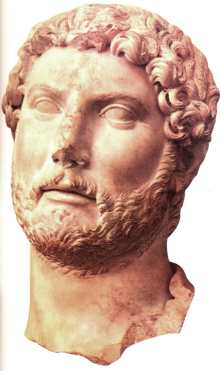
\includegraphics[height=.7\textheight]{images/publio.jpg}
   		\end{center}
   		\column{.6\textwidth}  		
   		\begin{block}{Frase}
   			\begin{center}
   				{\large O plano que não pode ser mudado não presta.}
   			\end{center}
   		\end{block}		  		
   		\begin{block}{Quem?}
   			\begin{center}
   				{\bf Públio Siro (??? - 43 d.C.)} \\Escritor latino da Roma antiga.
   			\end{center}
   		\end{block}
   	\end{columns}
   \end{frame}
    
    \section{Revisão}
	\subsection{Grafos Bipartidos}
	\begin{frame}{Grafo Bipartido}
		\begin{block}{Definição}
			Um grafo $G$ é {\bf bipartido} se existe uma bipartição $\{U, W \}$ de $V_G$ tal que toda aresta de $G$ tem uma ponta em $U$ e outra em $W$.
		\end{block}
		\begin{block}{Lembrando... Bipartição!}
			Uma bipartição de um conjunto $V$ é um par $\{U, W\}$ de conjuntos não vazios tal que $U \cup W = V$ e $U \cap W = \emptyset$.
		\end{block}
		\begin{block}{Notação}
			\begin{itemize}
				\item Para explicitar a partição, podemos dizer que o grafo é {\bf $\{ U, W \}$-bipartido}. 
				\item Se $G$ é um grafo $\{ U, W \}$-bipartido, podemos dizer, informalmente, que os elementos de $U$ são os {\bf vértices brancos} e os de $W$ são os {\bf vértices pretos} do grafo.
			\end{itemize}
		\end{block} 
	\end{frame}
	
	\begin{frame}{Grafo Bipartido}
		\begin{block}{Grafo $\{ U, W \}$-bipartido completo}
			Um grafo $\{U, W \}$-bipartido é {\bf completo} se todo vértice branco é adjacente a todos os vértices pretos. 
		\end{block}
		\begin{center}
			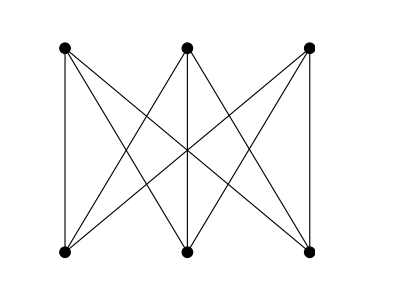
\includegraphics[width=.6\textwidth]{images/bipartido-completo.png}
		\end{center}
	\end{frame}
	
	\section{Grafo Bipartido (Cont.)}
	
	\begin{frame}{Grafo Bipartido}
		\begin{block}{$K_{p,q}$}
			Um $K_{p,q}$ é um grafo bipartido completo com \\$p$ vértices brancos e $q$ pretos.
		\end{block} \pause
		\begin{block}{Estrela}
			\begin{itemize}
				\item Uma {\bf estrela} é um grafo $K_{1,q}$; \pause
				\item Se $q \geq 2$, o {\bf centro} da estrela é o único vértice que incide em duas ou mais arestas; \pause
				\item Se $q < 2$, a estrela não tem centro.
			\end{itemize}
		\end{block}
	\end{frame}

	\section{Caminhos e Circuitos}
	\begin{frame}[shrink]{Caminhos e Circuitos}
		\begin{block}{Caminho}
			Um grafo $G$ é um {\bf caminho} se $V_G$ admite uma permutação $(v_1, v_2, \ldots , v_n)$ tal que
			\begin{center}
				$E_G = \{ v_i v_{i +1} : 1 \leq i < n \}$
			\end{center} \pause
			\begin{itemize}
				\item os vértices $v_1$ e $v_n$ são os {\bf extremos} do caminho; \pause
				\item os demais vértices são {\bf internos}; \pause
				\item diremos que esse caminho {\bf liga} $v_1$ a $v_n$.
			\end{itemize}
		\end{block} \pause
		\begin{block}{Notação}
			Podemos denotar um caminho pela sequência representada pelos seus vértices: \pause
			\begin{center}
				$v_1 v_2 \ldots v_n$		
			\end{center}
		\end{block}
	\end{frame}
	
	\begin{frame}[shrink]{Caminhos e Circuitos}
		\begin{block}{Circuito}
			Um grafo $G$ é um {\bf circuito} se $V_G$ tem 3 ou mais elementos e admite uma permutação $(v_1, v_2, \ldots , v_n)$ tal que
			\begin{center}
				$E_G = \{ v_i v_{i +1} : 1 \leq i < n \} \cup \{ v_1 v_n \}$
			\end{center} 
		\end{block} \pause
		\begin{block}{Notação}
			\begin{itemize}
				\item Podemos denotar um circuito simplesmente por: \pause
				\begin{center}
					$v_1 v_2 \ldots v_n v_1$		
				\end{center}
				\item O {\bf comprimento} de um caminho ou circuito $G$ é o número $m(G)$; \pause
				\item Um {\bf triângulo, quadrado, pentágono {e} hexágono} é o mesmo que um circuito de comprimento 3, 4, 5 e 6 respectivamente.
			\end{itemize}
		\end{block}
	\end{frame}
	
	\begin{frame}
		\titlepage
	\end{frame}
	
\end{document}